\documentclass[16pt]{beamer}

\title{Notre mouchard de poche}

\usetheme{default}

\usepackage[utf8]{inputenc}
\usepackage{amsmath}
\usepackage{amsfonts}
\usepackage{amssymb}
\usepackage{pgf}
\usepackage{color}
\usepackage[frenchb]{babel}
\usepackage{amssymb}
\usepackage{hyperref}

\usefonttheme{default}
\usepackage{DejaVuSans}
%\usepackage[sfdefault]{FiraSans} %% option 'sfdefault' activates Fira Sans as the default text font
\usepackage[T1]{fontenc}
\renewcommand*\oldstylenums[1]{{\firaoldstyle #1}}


\setbeamertemplate{navigation symbols}{} %remove navigation symbols

\author{Cédric Jeanneret (aka \href{https://www.twitter.com/SwissTengu}{@SwissTengu})}
\institute{\href{https://www.ethack.org/}{EthACK.org}}
\date{\today}

\definecolor{linecolor}{HTML}{4d4c4c}

\setbeamercolor{linecolor}{fg=white,bg=linecolor}

\setbeamertemplate{headline} {
	\begin{beamercolorbox}[wd=\paperwidth,dp=8pt,ht=12pt,leftskip=.29cm,rightskip=.29cm]{linecolor}
	\hfill
	\hypersetup{
		colorlinks=true,
		linkcolor=white,
		urlcolor=white,
	}
	\insertinstitute
	\end{beamercolorbox}%
}

\setbeamertemplate{footline}{%
	\begin{beamercolorbox}[wd=\paperwidth,dp=9pt,ht=0.4cm,leftskip=.29cm,rightskip=.3cm]{linecolor}
	\pgfputat{\pgfxy(0.455,-0.315)}{\pgfbox[center,base]{
\includegraphics[width=1.5cm]{../common/logo_537.png}}}
	\hfill
	\inserttitle
	\end{beamercolorbox}%
}


\hypersetup{
	colorlinks=true,
	linkcolor=blue,
	urlcolor=blue,
	pdfborderstyle={/S/U/W 1},
	pdfborder=0 0 1,
	linkbordercolor={0 0 0},
	urlbordercolor={0 0 0},
}


\begin{document}

{
\setbeamertemplate{footline}{%
	\begin{beamercolorbox}[wd=\paperwidth,dp=8pt,ht=12pt,leftskip=.29cm,rightskip=.3cm]{linecolor}
	\hfill
	\inserttitle
	\end{beamercolorbox}%
}

% center first slide — not a title, but almost
{
\centering
\begin{frame}

EthACK
\vspace{0.5cm}

The Swiss Privacy Basecamp 
\vspace{0.5cm}


\includegraphics[width=4cm]{../common/logo_537.png}

\end{frame}
}
}

\begin{frame}{EthACK ?}
\begin{itemize}
	\item Éthique
	\item État
	\item ACKnowledgement (reconnaissance)
	\item Hacking (éthique, évidemment)
	\item …
\end{itemize}
\end{frame}

\begin{frame}{Pourquoi ?}
\begin{itemize}
	\item Notre gouvernement ne s'intéresse pas (ou peu) au sujet
	\item Les sociétés privées nous fichent à notre insu
	\item Personne ne sait où sont leurs données, qui les traitent, à quoi elles servent
\end{itemize}
\end{frame}



\begin{frame}
  \titlepage
\end{frame}

\begin{frame}{Description de la menace}
\begin{itemize}
\item Vol de l'appareil
\item Applications ``indélicates''
\item Fournisseurs de services ``cloud''
\item Écoute au niveau de l'antenne GSM
\end{itemize}
\end{frame}

\begin{frame}{Smartphones vs Smartusers}
\begin{itemize}
\item Que sait notre smartphone ?
\item Comment mitiger ?
\item Applications disponibles
\item ROMS alternatives : bien, ou pas bien ?
\item Bonnes pratiques
\end{itemize}
\end{frame}

\begin{frame}{Quelques chiffres}
\begin{itemize}
\item \textcolor{red}{1.5 milliards} de smartphones dans le monde (2013)
\item Plus de \textcolor{red}{10 millions} de cartes SIM en Suisse (OFCOM 2012)
\item Plus de \textcolor{red}{75\%} des utilisateurs accèdent à Internet via leur smartphone (en Suisse)
\end{itemize}
\end{frame}

\begin{frame}{Quelques chiffres et faits}
\begin{itemize}
\item Plus de \textbf{16'600 To} de communications Internet depuis le réseau mobile (OFCOM 2012)
\item Chiffrement GSM cassé en 2009
\item La 2G ne valide pas l'antenne, que le client
\item Technologie \textgreater = 3G identifie les deux
\end{itemize}
\end{frame}

\begin{frame}{Xmbplfgrz ?!}
\begin{description}
\item[GSM] \hfill \\ standard ``2G'' (seconde génération), remplace ``1G'' (première génération)
\item[3G] \hfill \\ Troisième génération du standard
\item[Chiffrement] \hfill \\ brouiller le contenu à l'aide d'un ``chiffre'' (crypter dans les médias)
\end{description}
\begin{description}
\item[Le contraire de ``chiffrer''] \hfill \\ \textbf{déchiffrer}
\item[décrypter] \hfill \\ casser le chiffrement sans le chiffre
\end{description}
\end{frame}

\begin{frame}{Mais c'est sécurisé… Non ?}

\centering
Voui, bien sûr ;)
\vspace{0.5cm}

Les communications (SMS/Voix) sont \textcolor{red}{déchiffrées au niveau
de l'antenne}.
\vspace{0.5cm}

\textcolor{red}{\textbf{Y compris quand vous êtes à l'étranger}}
\end{frame}

{
\hypersetup{
	colorlinks=true,
	linkcolor=white,
	urlcolor=white
}
\setbeamertemplate{headline} {
	\begin{beamercolorbox}[wd=\paperwidth,dp=8pt,ht=12pt,leftskip=.29cm,rightskip=.29cm]{linecolor}
	Source: \textbf{\href{http://www.imdb.com/title/tt0067992/}{Willy Wonka \& the Chocolate Factory, 1971}}
	\hfill
	\insertinstitute
	\end{beamercolorbox}%
}
\begin{frame}
\centering

\includegraphics[width=\textwidth,height=\textheight,keepaspectratio]{./maxresdefault.jpg} 
\end{frame}
}



{
\hypersetup{
	colorlinks=true,
	linkcolor=white,
	urlcolor=white
}
\setbeamertemplate{headline} {
	\begin{beamercolorbox}[wd=\paperwidth,dp=8pt,ht=12pt,leftskip=.29cm,rightskip=.29cm]{linecolor}
	Source: \textbf{\href{https://en.wikipedia.org/wiki/GSM}{Wikipedia}}
	\hfill
	\insertinstitute
	\end{beamercolorbox}%
}
\begin{frame}
\centering
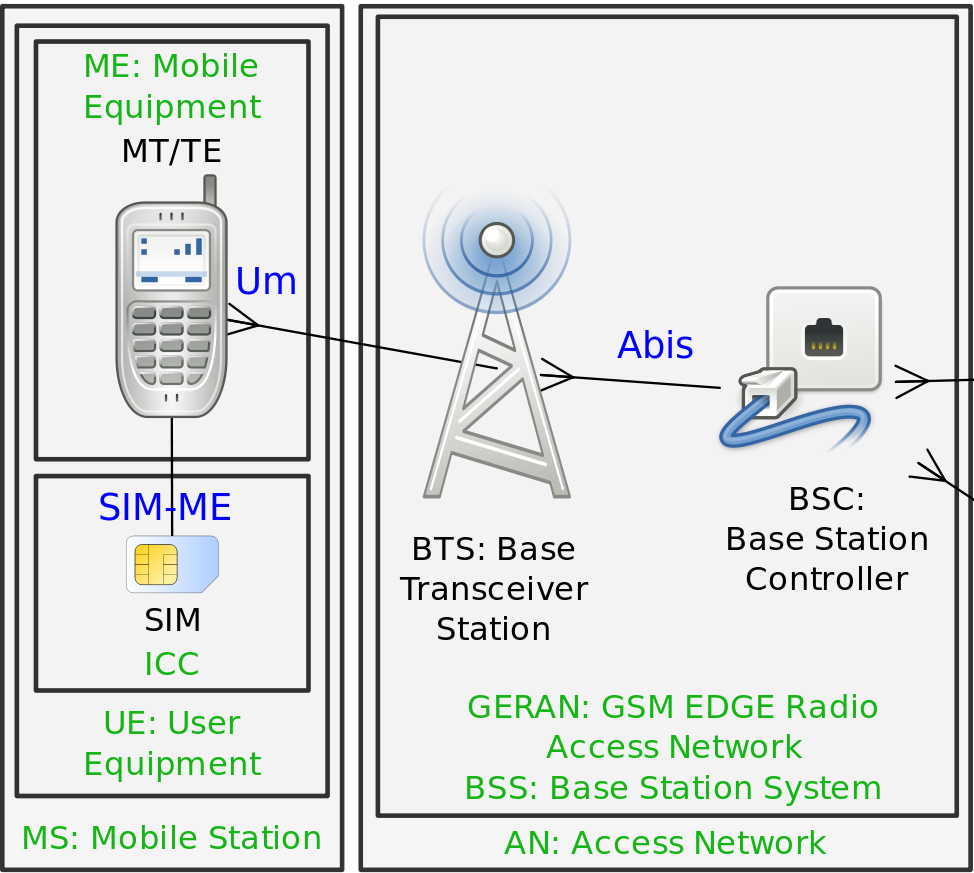
\includegraphics[width=\textwidth,height=\textheight,keepaspectratio]{./Gsm_structures.png} 
\end{frame}
}

\begin{frame}
{Rappelez-vous ;)}
\centering
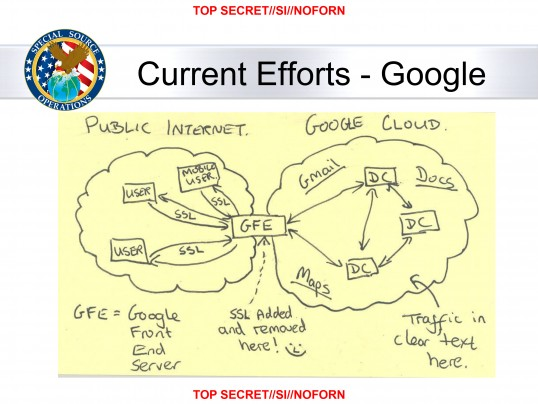
\includegraphics[width=\textwidth,height=\textheight,keepaspectratio]{./postitnote.jpg} 
\end{frame}


\begin{frame}{Smart, so smart}
\begin{itemize}
\item Localisation
\item Contacts
\item Données biométriques
\item Données médicales
\item Reconnaissance faciale
\item Intéractions numériques et humaines
\item \emph{OK Google, OK Glass, Siri}
\item Amazon \href{http://www.amazon.com/oc/echo/}{Echo} Voice Control System
\end{itemize}
\end{frame}

\begin{frame}{Capteurs}
\begin{description}
\item[Gyroscope] \hfill \\
Position dans l'espace
\item[Accéléromètre] \hfill \\
Direction du mouvement (et déduction vitesse)
\item[Écran tactile] \hfill \\
Manière de faire le \emph{swipe} et \emph{tap}
\item[Baromètre] \hfill \\
Données sur votre emplacement (altitude, conditions etc)
\end{description}
\end{frame}

\begin{frame}{Empreintes des capteurs}
\begin{description}
\item[Imprécisions au niveau des capteurs] \hfill \\
Permettent d'identifier l'appareil de manière \href{http://www.ece.illinois.edu/mediacenter/article.asp?id=7897}{précise et unique} (ECE ILLINOIS)
\item[Votre utilisation] \hfill \\
Permet de vous identifier de façon unique
\end{description}
\end{frame}

\begin{frame}{Biométrie et santé}
\begin{description}
\item[Des données qui ne peuvent pas changer] \hfill \\
\begin{itemize}
\item Sur un appareil qu'on peut perdre
\item Sur un appareil qui peut se faire voler
\item Sur un appareil configuré par défaut pour envoyer son contenu sur le Net
\item Vos empreintes couvrent l'appareil
\end{itemize}
\item[Données médicales] \hfill \\
Adieu, secret médical…
\end{description}
\end{frame}

\begin{frame}
{Données immuables servant de mot de passe}
\centering
``Suite à une fuite de données, merci de changer vos empreintes digitales''

\vspace{1cm}

Ou votre rétine…
\end{frame}

\begin{frame}{}
\centering
\textbf{On ne va pas se laisser faire tout de même !?}

\vspace{1cm}
Quelques préliminaires.
\end{frame}

\begin{frame}{Jamais le premier soir}
\begin{description}
\item[Commencer par trier les applications] \hfill \\
\begin{itemize}
\item Désactiver/désinstaller les applications inutiles
\item Attention aux ``packs fournisseurs''
\end{itemize}

\item[Éviter de s'enregistrer auprès des services ``remote''] \hfill \\
… même si c'est ``tellement pratique''
\end{description}

\end{frame}

\begin{frame}{Ni le second}
\begin{description}
\item[Attention aux permissions !] \hfill \\
\begin{itemize}
\item Est-ce qu'un \textcolor{red}{jeu} a réellement besoin d'accéder aux \emph{contacts} ?
\item Est-ce qu'un \textcolor{red}{calendrier} a réellement besoin de la \emph{localisation} ?
\item Est-ce qu'un \textcolor{red}{lecteur de musique} a réellement besoin du \emph{journal des appels} ?
\end{itemize}
\end{description}
\end{frame}

\begin{frame}{Sortez couverts}
\begin{description}
\item[Désactivez le GPS] \hfill \\
La plupart du temps, le GPS est inutile
\item[Désactivez le NFC] \hfill \\
Near Field Contact : ``utile'' pour paiement sans contact ou transferts, mais 99\% du temps inutile
\item[Désactivez Internet] \hfill \\
Apprenez à ne plus être connecté 100\% du temps. Votre batterie vous dira merci ;)
\item[Désactivez le Bluetooth] \hfill \\
Idem que pour le NFC.
\end{description}
\end{frame}

\begin{frame}{Pourquoi désactiver ?}
\begin{description}
\item[Batterie] \hfill \\
L'autonomie est déjà assez mauvaise (une journée) sans en rajouter…
\item[Publicité ciblée] \hfill \\
Des magasins utilisent déjà Internet et votre géolocalisation pour vous cibler
\item [NFC] \hfill \\
Votre appareil lit et peut être lu, transmettre/recevoir des données à votre insu, etc.
\item[Bluetooth] \hfill \\
Identité BT; bornes dans les magasins
\end{description}
\end{frame}

\begin{frame}
{Marketing on NFC}
\begin{description}
\item[\href{http://www.linkedin.com/in/alexdo1}{Alex Do} (Landor, Fab.com)] \hfill \\
``We could use NFC to push information to customers' mobiles as they walk through malls'' \\
\vspace{0.3cm}
``[…] they could use NFC to advertise digitally - to push deals, VIP invites, and announce new product releases to attract customers to their stores''
\end{description}
Source: \href{http://www.wpp.com/wpp/marketing/digital/what-nfc-can-do-for-brands/}{WPP} \\

Regardez aussi ``nfc marketing usage''…
\end{frame}

\begin{frame}{Donc on est fichu}
\centering
\textbf{Oui. Et fiché, surtout.}
\vspace{1.0cm}

\textcolor{red}{Mais on peut lutter.}
\end{frame}

\begin{frame}
{Se découpler des services centralisés}
\begin{description}
\item[Centralisation ?] \hfill \\
\emph{Une} entité possède \emph{toutes} vos données.
\item[Solution] \hfill \\
Employer différents services chez différents fournisseurs. \\
Si possible ``locaux'' (lois suisses, for juridique en Suisse, etc).
\end{description}
\end{frame}

\begin{frame}{Décentralisation — contacts et calendriers}
\begin{itemize}
\item \textbf{\href{https://whispersystems.org/blog/flock/}{Flock}} (opensource, possibilité d'employer le service payant)

\item \textbf{\href{http://davdroid.bitfire.at/what-is-davdroid}{DAVDroid}} (opensource, demande un hébergement spécialisé; compatible OwnCloud)

\end{itemize}
\end{frame}

\begin{frame}
{Décentralisation — fichiers}
\begin{itemize}
\item \textbf{\href{https://spideroak.com/}{Spider Oak}} (propriétaire, US; chiffrement côté client)
\item \textbf{\href{https://owncloud.org/}{OwnCloud}} (opensource, US; hébergement possible sur \href{https://owncloud.com/}{owncloud.com})
\item \textbf{\href{http://seafile.com/en/home/}{Seafile}} (opensource, Chine; hébergement possible sur \href{http://seafile.com/en/product/cloud_service/}{seafile.com})
\end{itemize}
… et plein d'autres solutions qui se développent tous les jours
\end{frame}


\begin{frame}
{Décentralisation — Mails}

Alternatives à gmail, hotmail et autres

\begin{itemize}
\item \textbf{\href{https://www.infomaniak.ch}{Infomaniak}} (Suisse; à partir de 24CHF/an)
\item \textbf{\href{https://tutanota.de/}{Tutanota}} (Allemagne; gratuit, ou offres "business")
\item \textbf{\href{https://www.protonmail.ch}{ProtonMail}} (Suisse; effet ``soufflé''… ?)
\item \textbf{\href{https://ethack.org/}{EthACK}} (Suisse; oui, on planche dessus)
\end{itemize}
\end{frame}

\begin{frame}
{Décentralisation — Messagerie instantanée}

Alternatives à GTalk, iChat, iMessages et autres

\begin{itemize}
\item \textbf{\href{https://guardianproject.info/apps/chatsecure/}{chatSecure}} (opensource; permet d'employer votre compte gmail ou autres XMPP/Jabber)

\item \textbf{\href{https://whispersystems.org/}{TextSecure/Signal}} (opensource; échange de messages à-la Whatsapp, chiffrés)

\item \textbf{\href{https://smssecure.org/}{SMSSecure}} (opensource; envoi de SMS chiffrés)

\item \textbf{\href{https://threema.ch/}{Threema}} (propriétaire; échange de messages à-la Whatsapp, chiffrés)

\end{itemize}
\end{frame}

\begin{frame}
{ROM alternatives}

\begin{description}
\item[ROM ?] (Read Only Memory) \hfill \\
Système d'exploitation installé sur le smartphone

\item[iOS ?] \hfill \\
À notre connaissance, possible uniquement pour Android.
\end{description}
\end{frame}

\begin{frame}
{Avantages de changer l'OS}

\begin{description}
\item[Libre] \hfill \\
Les ROM alternatives sont libres et ouvertes, avec de solides communautés

\item[Le choix] \hfill \\
Il y a une certaine quantité d'alternatives existantes

\item[Vous reprenez votre appareil en main] \hfill \\
En choisissant une ROM adaptée à vos besoins \\
En choisissant d'installer ou non Gapps \\
En évitant les ``packs opérateurs''
\end{description}
\end{frame}

\begin{frame}
{Inconvénients}
\begin{description}
\item[Garantie] \hfill \\
Il est possible que la garantie soit annulée

\item[Connaissances] \hfill \\
Flasher un appareil demande 2-3 connaissances de base

\item[Limitations du choix de l'appareil] \hfill \\
Pas pour tous les appareils Android (secureboot, etc)

\item[Droits] \hfill \\
On se retrouve avec des droits avancés — amis Virus, bonjour !
\end{description}
\end{frame}

\begin{frame}
{ROM ``reconnues''}
\begin{itemize}
\item \href{http://www.cyanogenmod.org/}{CyanogenMod}
\item \href{http://download.paranoidandroid.co/roms/}{ParanoidAndroid}
\item \href{http://slimroms.net/}{SlimROMs}
\item \href{http://aokp.co/}{AOKP}
\item \href{http://www.pac-rom.com/}{PAC-ROM}
\item \href{http://www.replicant.us/}{Replicant}
\end{itemize}
\end{frame}

\begin{frame}
{To flash or not to flash, that's the question}
\centering
Up to you folks ;)
\end{frame}

\begin{frame}
{Bonnes pratiques}
\begin{description}
\item[Bloquer l'écran] \hfill \\
En évitant la biométrie

\item[Chiffrer les données] \hfill \\
Évitez de perdre le mot de passe…

\item[Désactiver le superflu] \hfill \\
Applications, services, fonctionnalités

\end{description}
\end{frame}

\begin{frame}
{Bonnes pratiques}
\begin{description}
\item[Contrôler les permissions] \hfill \\
Même si on ne peut pas toujours les limiter

\item[Lire les Conditions Générales d'Utilisation] \hfill \\
Même si c'est indigeste

\item[Installer le strict nécessaire] \hfill \\
Avez-vous réellement besoin de l'application ``coussin péteur'' ?
\end{description}
\end{frame}

{
\hypersetup{
	colorlinks=true,
	linkcolor=white,
	urlcolor=white
}
\setbeamertemplate{headline} {
	\begin{beamercolorbox}[wd=\paperwidth,dp=8pt,ht=12pt,leftskip=.29cm,rightskip=.29cm]{linecolor}
	Source : \textbf{\href{https://play.google.com/store/apps/details?id=com.kauf.soundboard.baum.FartSoundBoard}{Google Play}}
	\hfill
	\insertinstitute
	\end{beamercolorbox}%
}
\setbeamertemplate{logo}{}
\begin{frame}
\centering
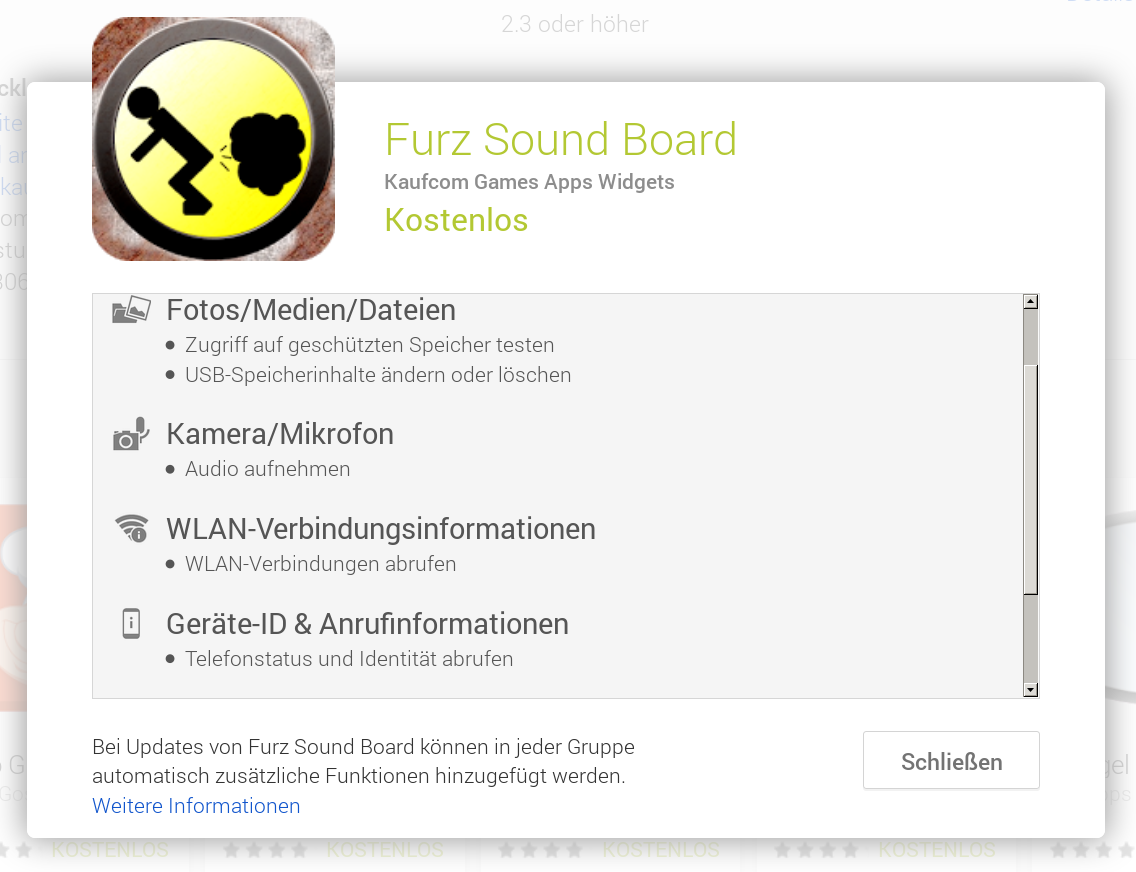
\includegraphics[width=\textwidth,height=\textheight,keepaspectratio]{./fartman.png}
\end{frame}
}

\begin{frame}
{Il existe deux choses qu'on ne peut pas limiter}

Qui peut :
\begin{itemize}
\item Accéder à toutes vos informations
\item Accéder à tous vos SMS
\item Accéder à tous vos appels
\item Exécute des commandes bas niveau
\item Posséder de multiples failles non-corrigées
\item Ne peut pas être mis à jour facilement pour appliquer des correctifs
\end{itemize}
\centering
\onslide<+->{\textbf{Une idée ?}}
\end{frame}

\begin{frame}
{Réponse}

\onslide<+->{}

\begin{description}
\onslide<+-> {
\item[Baseband] \hfill \\
\begin{itemize}
\item Très bas niveau dans l'appareil
\item Propriétaire, bardée de brevets
\item Déjà plusieurs preuves de vulnérabilités
\item Très bas niveau, donc dur à mettre à jour
\end{itemize}
}

\onslide<+-> {
\item[L'utilisateur] \hfill \\
\begin{itemize}
\item Ne réfléchit pas toujours
\item Adore cliquer sur tous les liens possibles
\item Adore installer tout et n'importe quoi
\item Fait rarement les mises à jour de son appareil
\end{itemize}
}

\end{description}
\end{frame}

\begin{frame}
{En résumé}
\centering
\textbf{Ne soyez pas plus bêtes que votre smartphone, et tout ira bien ;)}
\end{frame}


{
\setbeamertemplate{footline}{%
	\begin{beamercolorbox}[wd=\paperwidth,dp=8pt,ht=12pt,leftskip=.29cm,rightskip=.3cm]{linecolor}
	\hfill
	\inserttitle
	\end{beamercolorbox}%
}
{
\centering
\begin{frame}
{Questions ?}

\href{https://ethack.org/}{https://ethack.org/} \\
\vspace{0.3cm}
\href{https://www.twitter.com/EthACK_org}{@EthACK\_org} on Twitter \\
\vspace{0.3cm}
\href{https://www.facebook.com/ethack.org}{ethack.org} on Facebook

\vspace{0.5cm}


\includegraphics[width=4cm]{../common/logo_537.png}
\end{frame}
}
}

\end{document}
